\documentclass[10pt]{article}

\def\Type{LessonCaelan}
\def\TypeNum{Lesson 12}
\def\TypeTitle{Concavity \& The Second Derivative\\Key }
\def\Semester{Fall 2021} %Not Used 
\def\Course{MATH 1190 \& 1210}
\def\Targets{ {\bf\color{RedOrange}A1}, {\bf\color{RedOrange}A2} }

\usepackage{preambleDJ}

%%%%%%%%%%%% BEGIN DOCUMENT %%%%%%%%%%%%%%%
%%%%%%%%%%%% BEGIN DOCUMENT %%%%%%%%%%%%%%%
%%%%%%%%%%%% BEGIN DOCUMENT %%%%%%%%%%%%%%%
%%%%%%%%%%%% BEGIN DOCUMENT %%%%%%%%%%%%%%%
%%%%%%%%%%%% BEGIN DOCUMENT %%%%%%%%%%%%%%%



\begin{document}

\pagestyle{otherpages}
\thispagestyle{firstpage}
\vs{.6}

\textbf{Intended Learning Outcomes}
After this lesson, you will be able to 

\begin{itemize}
    \item Describe the meaning of concave up/down graphically and using the second derivative. (\target{A1})
    \item Identify concave up/down intervals and inflection points of a function from given graph or formula. (\target{A1})
    \item Represent concepts such as second derivative, concavity, and inflection points graphically. (\target{A1})
    \item Apply the Second Derivative Test to determine the local extrema of a function graphically and algebraically. (\target{A2})
\end{itemize}

\vspace{-0.5cm}

\hrulefill\\


{\bf\color{blue} Warm-up exercise 1.} Describe the relationship between a function $f$, tangent lines, $f^{\prime\prime}$ and ``bendiness" (an informal description of how $f$ is bending).\\



\fbox{
\begin{minipage}{0.95\textwidth}
\mpageT{.55}{.45}{
{\em Concave up} for $x$ on an interval $I$:
\itemI{
\item ``Bendiness": \blue{$f$ is bending up}
\item Tangent lines:  \blue{ are below the graph  of $f$.}
\item Derivative $f^{\prime}(x)$ is \blue{increasing}
\item $\ds f^{\prime\prime}(x)=\frac{d}{dx}[f^{\prime}(x)]\blue{>}0$ \blue{(positive)} 
}
}{
%
\,\hfill 
\includegraphics[width=0.4\textwidth]{images/concavity(2).PNG} \hfill 
\includegraphics[width=0.4\textwidth]{images/concavity(3).PNG} \hfill\,
}
\end{minipage}
}\\[0.1in]
%
\fbox{
\begin{minipage}{0.95\textwidth}
\mpageT{.55}{.45}{
{\em Concave down}  for $x$ on an interval $I$:
\itemI{
\item ``Bendiness": \blue{$f$ is bending down}
\item Tangent lines: \blue{ are above the graph  of $f$.}
\item Derivative $f^{\prime}(x)$ is \blue{decreasing}
\item $\ds f^{\prime\prime}(x)=\frac{d}{dx}[f^{\prime}(x))]\blue{<}0$ \blue{(negative)} 
}
}{
\,\hfill 
\includegraphics[width=0.4\textwidth]{images/concavity(1).PNG} \hfill 
\includegraphics[width=0.4\textwidth]{images/concavity(4).PNG} \hfill\,
}
\end{minipage}
}\\[0.1in]
%
\fbox{
\begin{minipage}{0.95\textwidth}
\mpageT{.55}{.45}{
{\em Inflection point}  at $x$:
\itemI{
\item Concavity \blue{changes sign}
\item $f^{\prime\prime}(x)=\blue{0}$ \blue{ or undefined}
}
\blue{It's not enough to say$f^{\prime\prime}(x)=0$  identifies locations of inflection points.   $f^{\prime\prime}(x)=0$ provides {\em  candidates} for inflection points but we must also confirm a change in sign of concavity before we can saty for sure. }
}{
\,\hfill 
\includegraphics[width=0.4\textwidth]{images/inflectionpoint.PNG} \hfill\,
}
\end{minipage}
}\\
\newpage
{\bf\color{blue}Warm-up exercise 2.}\ltrm{\color{RedOrange}A1} Identify which intervals $f$ would be {\it concave down} and inflection points if...\\
\mpageTth{.33}{.33}{.33}[\hs{.1}][\hs{.1}]{
\enumA{\item the curve pictured below were the graph of $f$?}\vs{-.2}
\begin{center}
    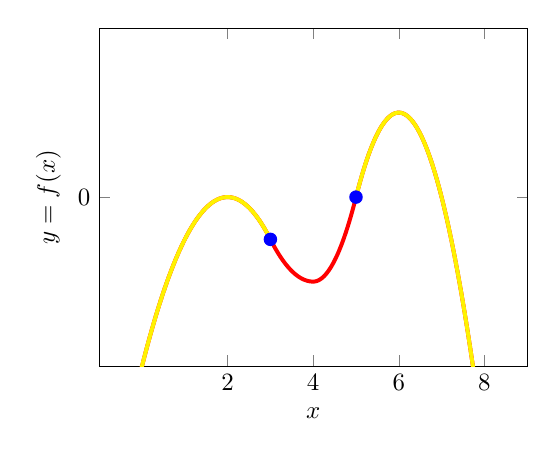
\begin{tikzpicture}[scale=.9]
          \begin{axis}[
            xlabel={$x$},
            ylabel={$y=f(x)$},
            %grid = major,
            xtick       = {2,4,6,8},
            xticklabels = {$2$,$4$,$6$,$8$},
            ytick       = {0},
            yticklabels = {$0$},
            samples     = 320,
            domain      = -1:9,
            restrict y to domain=-40:40,
            xmin = -1, xmax = 9,
            ymin = -4, ymax = 4,
            height=2.5in, width=3in
          ]
          \addplot[domain=-1:3, ultra thick, red] {-(x-2)^2};
          \addplot[domain=3:4, ultra thick, red] {(x-4)^2-2};
          \addplot[domain=4:5, ultra thick, red] {2*(x-4)^2-2};
          \addplot[domain=5:9, ultra thick, red] {-2*(x-6)^2+2};
           \addplot[domain=-1:3, ultra thick, yellow] {-(x-2)^2};
           \addplot[domain=5:9, ultra thick, yellow] {-2*(x-6)^2+2};
            \filldraw[blue] (3,-1) circle (2.5pt);
            \filldraw[blue] (5,0) circle (2.5pt);
          %
        \end{axis}
    \end{tikzpicture}
\end{center}
}{
\enumA{\setItemnumber{2}\item the curve pictured below were the graph of $f'$?}\vs{-.2}
\begin{center}
    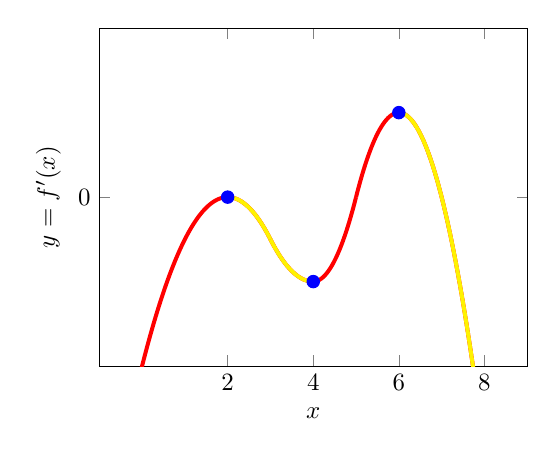
\begin{tikzpicture}[scale=.9]
          \begin{axis}[
            xlabel={$x$},
            ylabel={$y=f^{\prime}(x)$},
            %grid = major,
            xtick       = {2,4,6,8},
            xticklabels = {$2$,$4$,$6$,$8$},
            ytick       = {0},
            yticklabels = {$0$},
            samples     = 320,
            domain      = -1:9,
            restrict y to domain=-40:40,
            xmin = -1, xmax = 9,
            ymin = -4, ymax = 4,
            height=2.5in, width=3in
          ]
          \addplot[domain=-1:3, ultra thick, red] {-(x-2)^2};
          \addplot[domain=3:4, ultra thick, red] {(x-4)^2-2};
          \addplot[domain=4:5, ultra thick, red] {2*(x-4)^2-2};
          \addplot[domain=5:9, ultra thick, red] {-2*(x-6)^2+2};
		\addplot[domain=2:3, ultra thick, yellow] {-(x-2)^2};
		\addplot[domain=3:4, ultra thick, yellow] {(x-4)^2-2};
		\addplot[domain=6:9, ultra thick, yellow] {-2*(x-6)^2+2};
		\filldraw[blue] (2,0) circle (2.5pt);
		\filldraw[blue] (4,-2) circle (2.5pt);
		\filldraw[blue] (6,2) circle (2.5pt);
          %
        \end{axis}
    \end{tikzpicture}
\end{center}
}{
\enumA{\setItemnumber{3}\item the curve pictured below were the graph of $f''$?}\vs{-.2}
\begin{center}
    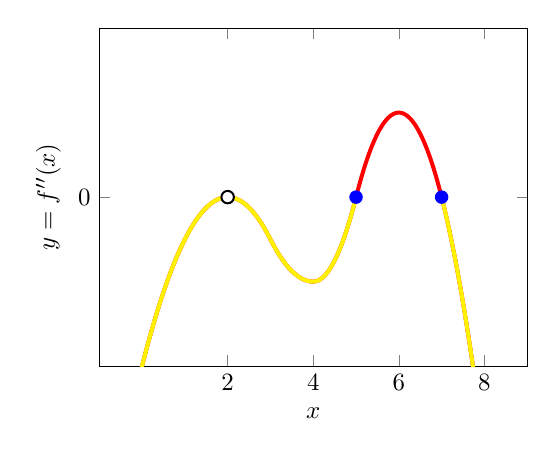
\begin{tikzpicture}[scale=.9]
          \begin{axis}[
            xlabel={$x$},
            ylabel={$y=f^{\prime \prime}(x)$},
            %grid = major,
            xtick       = {2,4,6,8},
            xticklabels = {$2$,$4$,$6$,$8$},
            ytick       = {0},
            yticklabels = {$0$},
            samples     = 320,
            domain      = -1:9,
            restrict y to domain=-40:40,
            xmin = -1, xmax = 9,
            ymin = -4, ymax = 4,
            height=2.5in, width=3in
          ]
          \addplot[domain=-1:3, ultra thick, red] {-(x-2)^2};
          \addplot[domain=3:4, ultra thick, red] {(x-4)^2-2};
          \addplot[domain=4:5, ultra thick, red] {2*(x-4)^2-2};
          \addplot[domain=5:9, ultra thick, red] {-2*(x-6)^2+2};
		\addplot[domain=-1:3, ultra thick, yellow] {-(x-2)^2};
		\addplot[domain=3:4, ultra thick, yellow] {(x-4)^2-2};
		\addplot[domain=4:5, ultra thick, yellow] {2*(x-4)^2-2};
		\addplot[domain=7:9, ultra thick, yellow] {-2*(x-6)^2+2};
		  \filldraw[white] (2,0) circle (2.5pt);
		\draw[thick] (2,0) circle (2.5pt);
		\filldraw[blue] (5,0) circle (2.5pt);
		\filldraw[blue] (7,0) circle (2.5pt);          %
        \end{axis}
    \end{tikzpicture}
\end{center}
}
\mpageTth{.33}{.33}{.33}[\hs{.1}][\hs{.1}]{
\sol{
\itemI{
\item {\em Concavity}
Given a graph of $f(x)$ we look where ``bendiness" is down. This occurs on
$(-\infty,3),\,(5,\infty)$. 
\item {\em Inflection points}.  
\itemC{
\item The concavity changes from down to up at $x=3$ and thus $f^{\prime\prime}(x)$ changes sign and $x=3$ is an inflection point.
\item The concavity changes from up to down at $x=5$ and thus $f^{\prime\prime}(x)$ changes sign and $x=5$ is an inflection point.
}
}
}
}{
\sol{
\itemI{
\item {\em Concavity}
Given a graph of $f^{\prime}(x)$ we look where $f^{\prime}$ is decreasing which means $\ds \frac{d}{dx}[f^{\prime}(x)]=f^{\prime\prime}(x)<0$.  This occurs on
$(2,4),\, (6,\infty)$. 
\item {\em Inflection points} 
\itemC{
\item Before $x=2$, $f^{\prime}$ is increasing and thus $f^{\prime\prime}>0$. After $x=2$,  $f^{\prime}$ is decreasing and thus $f^{\prime\prime}<0$, Since the sign of $f^{\prime\prime}$ changes, $x=2$ is an inflection point.
\item  Before $x=4$, $f^{\prime}$ is decreasing and thus $f^{\prime\prime}<0$. After $x=4$,  $f^{\prime}$ is increasing and thus $f^{\prime\prime}>0$, Since the sign of $f^{\prime\prime}$ changes, $x=4$ is an inflection point.
\item Before $x=6$, $f^{\prime}$ is increasing and thus $f^{\prime\prime}>0$. After $x=6$,  $f^{\prime}$ is decreasing and thus $f^{\prime\prime}<0$, Since the sign of $f^{\prime\prime}$ changes, $x=6$ is an inflection point.
}
 \item We do not include $x=2$, $x=4$, nor $x=6$ in our concave up/down intervals since $f^{\prime\prime}(x)=0$ at those points. 
}
}
}{
\sol{
\itemI{
\item {\em Concavity}
Given a graph of $f^{\prime\prime}(x)$ we look where $f^{\prime\prime}<0$.  This occurs on
$(-\infty, 2),\, (2,5),\, (7,\infty)$.
\item {\em Inflection points}.  Candidates for inflection points occur when $f^{\prime\prime}(x)=0$ or when $f^{\prime\prime}(x)$ is undefined.  Based on the graph of $f^{\prime\prime}(x)$ above, $f^{\prime\prime}(x)=0$ when $x=2$, $x=5$ and $x=7$.
\itemC{
\item Just before $x=2$, $f^{\prime\prime}(x)<0$.  Just after $x=2$, $f^{\prime\prime}(x)<0$. Since $f^{\prime\prime}(x)$ does not change sign, $x=2$ {\em is not} an inflection point.
\item Just before $x=5$, $f^{\prime\prime}(x)<0$.  Just after $x=5$, $f^{\prime\prime}(x)>0$. Since $f^{\prime\prime}(x)$  changes sign, $x=5$ {\em is} an inflection point.
\item Just before $x=7$, $f^{\prime\prime}(x)>0$.  Just after $x=7$, $f^{\prime\prime}(x)<0$. Since $f^{\prime\prime}(x)$  changes sign, $x=7$ {\em is} an inflection point.
}
\item  We do not include $x=2$, $x=5$, nor $x=7$ in our concave up/down intervals since $f^{\prime\prime}(x)=0$. 
}
}
}

%%%%%%%%
\newpage%
%%%%%%%%

{\bf\color{blue}Mini-lecture.}  Last time, we located local extrema using the First Derivative Test. Today,  we {\em locate local extrema using the Second Derivative Test}.\\
\mpageTfour{.25}{.25}{.25}{.25}{
\blue{
\hs{-.3}
\itemC{
\item At $(c,f(c))$ we have flat tangent line, so $f^{\prime}(c)=0$. 
\item Additionally, we see yellow part of graph is concave down, so $f^{\prime\prime}(c)<0$
\item We also have a local maximum at this location.
\item All of this leads us to statement (a) in the Second Derivative Test.
}
}
}{\centering
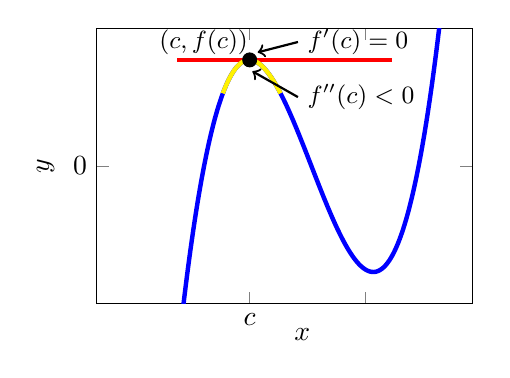
\begin{tikzpicture}[scale=1]
          \begin{axis}[
            xlabel={$x$},
            xlabel style={anchor=west},
            ylabel={$y$}, 
            ylabel style={anchor=south},
            %grid = major,
            xtick       = {1.85,4,6,8},
            xticklabels = {$c$,,,},
            ytick       = {0},
            yticklabels = {$0$},
            samples     = 320,
            domain      = -1:6,
            restrict y to domain=-40:40,
            xmin = -1, xmax = 6,
            ymin = -4, ymax = 4,
            height=2in, width=2.5in
          ]
          % old version of the curve
          %
          %\addplot[domain=-1:9, purple, ultra thick, mark=none] {-1/10*(x-1)*(x-4)^2*(x-7)};
          %
          %new version of the curve in pieces
          %
          \addplot[domain=0:6, ultra thick, blue] {((x-1)*(x-3)*(x-5)};
          \addplot[domain=0.5:4.5, ultra thick, red] {3.08};
          \addplot[domain=01.35:2.425, ultra thick, yellow] {((x-1)*(x-3)*(x-5)};
            \filldraw (1.85,3.08) circle (2.5pt);
            \node[anchor=west] at (2.75,2) {\small $f^{\prime\prime}(c)<0$};
            \draw[thick, ->] (2.75,2) -- (1.9,2.75);
             \node[anchor=west] at (2.75,3.6) {\small $f^{\prime}(c)=0$};
		 \draw[thick, ->] (2.75,3.6) -- (2,3.3);
		 \node[anchor=east] at (2,3.6) {\small $(c,f(c))$};
          %
        \end{axis}
    \end{tikzpicture}
\captionof*{figure}{\bf Local Maximum}
}{
\mpageT{.2}{.9}{
\mbox{}
}{
\blue{
\hs{-.3}
\itemC{
\item At $(c,f(c))$ we have flat tangent line, so $f^{\prime}(c)=0$. 
\item Additionally, we see yellow part of graph is concave up, so $f^{\prime\prime}(c)>0$
\item We also have a local minimum at this location.
\item All of this leads us to statement (b) in the Second Derivative Test.
}
}
}
}{\centering
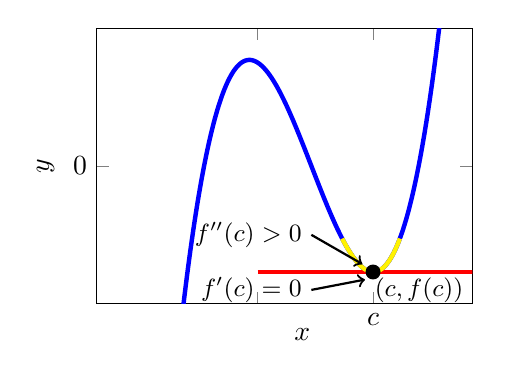
\begin{tikzpicture}[scale=1]
          \begin{axis}[
            xlabel={$x$},
            xlabel style={anchor=west},
            ylabel={$y$}, 
            ylabel style={anchor=south},
            %grid = major,
            xtick       = {2,4.15,6,8},
            xticklabels = {,$c$,,},
            ytick       = {0},
            yticklabels = {$0$},
            samples     = 320,
            domain      = -1:6,
            restrict y to domain=-40:40,
            xmin = -1, xmax = 6,
            ymin = -4, ymax = 4,
            height=2in, width=2.5in
          ]
          \addplot[domain=0:6, ultra thick, blue] {((x-1)*(x-3)*(x-5)};
          \addplot[domain=2:6, ultra thick, red] {-3.08};
          \addplot[domain=3.575:4.65, ultra thick, yellow] {((x-1)*(x-3)*(x-5)};
            \filldraw (4.15,-3.08) circle (2.5pt);
            \node[anchor=east] at (3,-2) {\small $f^{\prime\prime}(c)>0$};
            \draw[thick, ->] (3,-2) -- (3.95,-2.85);
             \node[anchor=east] at (3,-3.6) {\small $f^{\prime}(c)=0$};
	\draw[thick, ->] (3,-3.6) -- (4,-3.3);
	 \node[anchor=west] at (4,-3.6) {\small $(c,f(c))$};
          %
        \end{axis}
    \end{tikzpicture}
\captionof*{figure}{\bf Local Minimum}
}


\important{Second Derivative Test}
{
Suppose $f''$ is continuous near a critical number $x=c$. \blue{(i.e. $f^{\prime}(c)=0$ or $f^{\prime}(c)=DNE$)} 
\enumA{
\item If \blue{$f^{\prime}(c)=0$ and $f^{\prime\prime}(c)<0$ then we have Local Maximum at $x=c$} \hfill  Local Maximum at $x=c$\\
\item  If \blue{$f^{\prime}(c)=0$ and $f^{\prime\prime}(c)>0$ then we have Local Minimum at $x=c$}  \hfill  Local Minimum at $x=c$\\
\item If  \blue{$f^{\prime}(c)=DNE$ then we cannot use the Second Derivative Test } \hfill Second Derivative Test is inconclusive.\\
}
}
\newpage
{\example} Let $g(x)=\dfrac{1}{x^2+1}$. $g^{\prime}(x)=\dfrac{-2x}{(x^2+1)^2}$ and $g^{\prime\prime}(x)=\dfrac{6x^2-2}{(x^2+1)^3}$.
\enumA{
\item\ltrm{\color{RedOrange}A1} Find the intervals on which $g$ is concave up and on which $g$ is concave down. Does the graph of $g$ have any inflection points? If so, then specify their $x$-coordinates. If not, then explain.
}
\sol{
We will create a sign line to help us decide where $g$ is concave up (CCU) and concave down (CCD). We will start by finding $g^{\prime\prime}(x)=0$. This will split up the domain into intervals where $g^{\prime\prime}>0$ or $g^{\prime\prime}<0$.
}
\blue{
\mpageT{.5}{.5}{\vs{-.2}
\al{
g^{\prime\prime}(x)&=0\\
\dfrac{6x^2-2}{(x^2+1)^3}&=0\\
\intertext{If the numerator is $0$, then the fraction will be too.}
6x^2-2&=0\\
6x^2&=2\\x^2&=\frac{2}{6}\\
x^2&=\frac{1}{3}\\
x&=\pm \sqrt{1/3}\\
x&=\pm \frac{1}{\sqrt{3}}
}
}{
A sign line captures what we have so far: \\
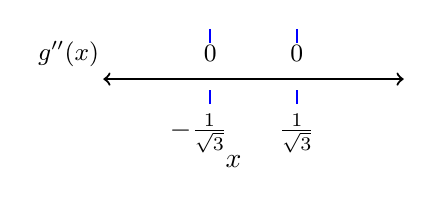
\begin{tikzpicture}[scale=1]
              \begin{axis}[
            xlabel={$x$},
            ylabel={},
            xlabel style={anchor=west},
	  y axis line style={draw opacity=0},
	  	  x axis line style={draw opacity=0},
            %grid = major,
            every major tick/.append style={ thick, blue, major tick length=5pt},
            xtick       = {-.577,.577},
            xticklabels = {$-\frac{1}{\sqrt{3}}\;\;\;$ , $\frac{1}{\sqrt{3}}$},
            ytick       = \empty,
            yticklabels={},
            samples     = 320,
            domain      = -2:2,
            restrict y to domain=-40:40,
            xmin = -3, xmax = 2,
            ymin = -.5, ymax = 1,
            height=1in, width=2.5in
          ]
	\draw[thick,<->] (-2,0) -- (2,0);
	 \node[anchor=west] at (-3,.5) {\small $g^{\prime\prime}(x)$};
	  \node at (-.577,.5) {\small $0$};
	   \node at (.577,.5) {\small $0$};
          %
        \end{axis}
    \end{tikzpicture}
    We will choose a point in the remaining intervals and test to see if $g^{\prime\prime}$ is positive or negative and thus CCU or CCD.  
\itemI{
\item Choose any $\ds x<-\frac{1}{\sqrt{3}}\approx -.577$, say $x=-1$. $\ds g^{\prime\prime}(-1)=\frac{6(-1)^2-2}{((-1)^2+1)^3}=\frac{4}{8}>0$
 \item Choose any $\ds x>\frac{1}{\sqrt{3}}\approx .577$, say $x=1$. $\ds g^{\prime\prime}(1)=\frac{6(1)^2-2}{((1)^2+1)^3}=\frac{4}{8}>0$
 \item Choose any $\ds -\frac{1}{\sqrt{3}}<x< \frac{1}{\sqrt{3}}$, say $x=0$. $\ds g^{\prime\prime}(0)=\frac{6(0)^2-2}{((0)^2+1)^3}=\frac{-2}{1}<0$
}
}\vs{.2}~\\
We update our sign line:
\begin{center}
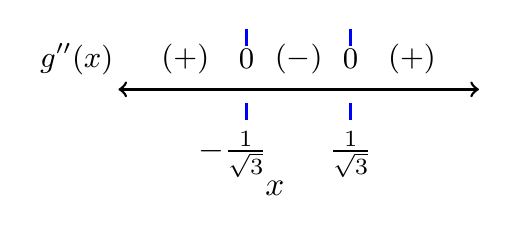
\begin{tikzpicture}[scale=1.2]
              \begin{axis}[
            xlabel={$x$},
            ylabel={},
            xlabel style={anchor=west},
	  y axis line style={draw opacity=0},
	  	  x axis line style={draw opacity=0},
            %grid = major,
            every major tick/.append style={ thick, blue, major tick length=5pt},
            xtick       = {-.577,.577},
            xticklabels = {$-\frac{1}{\sqrt{3}}\;\;\;$ , $\frac{1}{\sqrt{3}}$},
            ytick       = \empty,
            yticklabels={},
            samples     = 320,
            domain      = -2:2,
            restrict y to domain=-40:40,
            xmin = -3, xmax = 2,
            ymin = -.5, ymax = 1,
            height=1in, width=2.5in
          ]
	\draw[thick,<->] (-2,0) -- (2,0);
	 \node[anchor=west] at (-3,.5) {\small $g^{\prime\prime}(x)$};
	  \node at (-.577,.5) {\small $0$};
	   \node at (.577,.5) {\small $0$};
		\node at (-1.2577,.5) {\small $(+)$};
		\node at (1.2577,.5) {\small $(+)$};
		\node at (-0,.5) {\small $(-)$};
          %
        \end{axis}
    \end{tikzpicture}
\end{center}
We now see:
\itemI{
\item Intervals where $g$ is concave up: $(-\infty,-1/\sqrt{3}),( 1/\sqrt{3},\infty)$
\item Interval where $g$ is concave down: $(-1\sqrt{3},1/\sqrt{3})$
\item Since sign of $g^{\prime\prime}$ changes at $\ds x=-\frac{1}{\sqrt{3}}$ and $\ds x=\frac{1}{\sqrt{3}}$, these are both locations of inflection points. 
}
Other candidates for inflection points occur when $g^{\prime\prime}(x)=\dfrac{6x^2-2}{(x^2+1)^3}=DNE$.  The good news is that we will never have a division by $0$, $\sqrt{(-)}$, etc. and $g^{\prime\prime}$ is defined everywhere. Thus the only candidates for inflection points in this problem have already been found.
}

\enumA{\setItemnumber{2}
\item\ltrm{\color{RedOrange}A2} Recall that the only critical number of $g$ was $x=0$, with $g'(0)=0$. What does the Second Derivative Test tell us about the behavior of $g$ at its critical numbers?
}
 
 \sol{
 Since $g^{\prime}(0)=0$ it is a candidate for a Local Max or Local Min. Since $g^{\prime\prime}(0)<0$, then the Second Derivative Test tells us that we have a Local Maximum.
 } 
    
\newpage

{\exercise} Let $f(x)=\dfrac{x}{x^2+1}$.
\enumA{
\item\ltrm{\color{RedOrange}A1} Find the critical numbers of $f$.
\sol{We start with:
\al{
f^{\prime}(x)&=0?
\intertext{We will start with Quotient Rule since our function is in the form $\ds f(x)=\frac{\hi{(x)}}{\lo{(x)}}$ with $\hi{(x)}=x$ and $\lo{(x)}=x^2+1$ }
\frac{1\cdot(x^2+1)-x\cdot(2x)}{(x^2+1)^2}&=0\\
\frac{1-x^2}{(x^2+1)^2}&=0
\intertext{If the numerator $=0$ then $f^{\prime}(x)=0$}
1-x^2&=0\\
(1-x)(1+x)&=0
}
Thus $x=1$ and $x=-1$ are critical numbers. \\\\
We also check to see when $f^{\prime}(x)=DNE$. Since $\ds f^{\prime}(x)=\frac{1-x^2}{(x^2+1)^2}$ is defined everywhere (i.e. no division by $0$, no $\sqrt{(-)}$, etc.) we have found all of our critical numbers above.
}

\newpage
\item\ltrm{\color{RedOrange}A1} Given $f''(x)=\dfrac{2x(x+\sqrt3)(x-\sqrt3)}{(x^2+1)^3}$, find the intervals of $x$-values on which $f$ is concave up and on which $f$ is concave down.

\sol{
In order to find the intervals for which $f$ is concave up/down, we will build a sign line by finding }
\blue{
\mpageT{.5}{.5}[\vline]{\vs{-.15}
\al{
 f^{\prime\prime}(x)&=0\\
 \dfrac{2x(x+\sqrt3)(x-\sqrt3)}{(x^2+1)^3}&=0
 \intertext{We again focus on the numerator}
 2x(x+\sqrt3)(x-\sqrt3)&=0
 \intertext{This gives us 3 possibilities to test}
 2x=0&\Rightarrow x=0\\
 x+\sqrt3=0&\Rightarrow x=-\sqrt3\\
 x-\sqrt3=0&\Rightarrow x=\sqrt3
 }
Our sign line becomes
\begin{center}
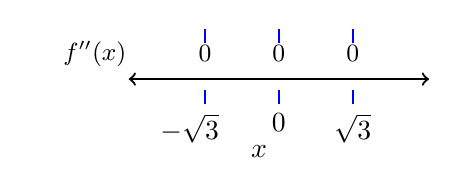
\begin{tikzpicture}[scale=1]
              \begin{axis}[
              axis line style={-},
              axis y line=left,
            xlabel={$x$},
            ylabel=\empty,
            xlabel style={anchor=west},
	  y axis line style={draw=none},
	  	  x axis line style={draw opacity=0},
            %grid = major,
            every major tick/.append style={ thick, blue, major tick length=5pt},
            xtick       = {-1.72, 0, 1.72},
            xticklabels = {$-\sqrt{3}\;\;\;\;$ ,$0$,  $\sqrt{3}$},
            ytick       = \empty,
            yticklabels={},
            samples     = 320,
            restrict y to domain=-40:40,
            xmin = -5.25, xmax = 3.5,
            ymin = -.5, ymax = 1,
            height=1in, width=2.5in
          ]
	\draw[thick,<->] (-3.5,0) -- (3.5,0);
	 \node[anchor=west] at (-5.25,.5) {\small $f^{\prime\prime}(x)$};
	  \node at (-1.72,.5) {\small $0$};
	  	   \node at (0,.5) {\small $0$};
	   \node at (1.72,.5) {\small $0$};
%		\node at (-1.2577,.5) {\small $(+)$};
%		\node at (1.2577,.5) {\small $(+)$};
%		\node at (-0,.5) {\small $(-)$};
          %
        \end{axis}
    \end{tikzpicture}
\end{center}
We now test a point in each interval to determine if $f$ is concave up/down in that interval
\itemI{
\item We pick a point $x<-\sqrt{3}\approx -1.72$, say $x=-2$. 
\al{
 f^{\prime\prime}(-2)&=\dfrac{2(-2)(-2+\sqrt3)(-2-\sqrt3)}{((-2)^2+1)^3}\\
 &=\frac{-4 (-2+\sqrt{3})(-2-\sqrt3)}{125}
 \intertext{We focus on the sign of each term}
 &=\frac{(-4)(-)(-)}{(+)}\\
 &=(-)
}
}
}{
\itemI{
\item  We pick a point $-\sqrt{3}\approx -1.72<x<0$, say $x=-1$. 
\al{
 f^{\prime\prime}(-1)&=\dfrac{2(-1)(-1+\sqrt3)(-1-\sqrt3)}{((-1)^2+1)^3}\\
 &=\frac{-1 (-1+\sqrt{3})(-1-\sqrt3)}{8}
 \intertext{We focus on the sign of each term}
 &=\frac{(-2)(+)(-)}{(+)}\\
 &=(+)
}
\item  We pick a point $0<x<\sqrt{3}\approx 1.72$, say $x=1$. 
\al{
 f^{\prime\prime}(1)&=\dfrac{2(1)(1+\sqrt3)(1-\sqrt3)}{((-1)^2+1)^3}\\
 &=\frac{1 (1+\sqrt{3})(1-\sqrt3)}{8}
 \intertext{We focus on the sign of each term}
 &=\frac{(+1)(+)(-)}{(+)}\\
 &=(-)
}
\item  We pick a point $x>\sqrt{3}\approx 1.72$, say $x=2$. 
\al{
 f^{\prime\prime}(2)&=\dfrac{2(2)(2+\sqrt3)(2-\sqrt3)}{((2)^2+1)^3}\\
 &=\frac{1 (1+\sqrt{3})(1-\sqrt3)}{125}
 \intertext{We focus on the sign of each term}
 &=\frac{(+2)(+)(+)}{(+)}\\
 &=(+)
}
}
}
We update our sign line:
\begin{center}
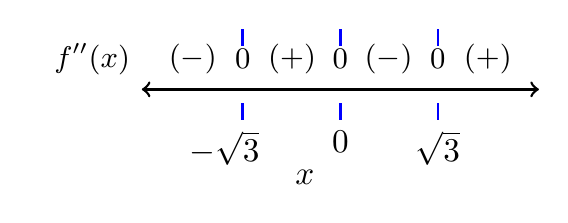
\begin{tikzpicture}[scale=1.2]
              \begin{axis}[
              axis y line=left,
            xlabel={$x$},
            ylabel={},
            xlabel style={anchor=west},
	  y axis line style={draw=none},
	  	  x axis line style={draw opacity=0},
            %grid = major,
            every major tick/.append style={ thick, blue, major tick length=5pt},
            xtick       = {-1.72, 0, 1.72},
            xticklabels = {$-\sqrt{3}\;\;\;\;$ ,$0$,  $\sqrt{3}$},
            ytick       = \empty,
            yticklabels={},
                                      y  axis line style=-,
                          % y axis/.append style={y axis line style=-}
            samples     = 320,
            restrict y to domain=-40:40,
            xmin = -5.5, xmax = 3.5,
            ymin = -.5, ymax = 1,
            height=1in, width=2.75in
          ]
	\draw[thick,<->] (-3.5,0) -- (3.5,0);
	 \node[anchor=west] at (-5.25,.5) {\small $f^{\prime\prime}(x)$};
	  \node at (-1.72,.5) {\small $0$};
	  	   \node at (0,.5) {\small $0$};
	   \node at (1.72,.5) {\small $0$};
		\node at (-2.6,.5) {\small $(-)$};
		\node at (-.85,.5) {\small $(+)$};
		\node at (.85,.5) {\small $(-)$};
		\node at (2.6,.5) {\small $(+)$};
          %
        \end{axis}
    \end{tikzpicture}
\end{center}
\itemI{
\item Concave up intervals: $(-\sqrt{3},0),\,(\sqrt{3},\infty)$
\item Concave down intervals: $(-\infty, -\sqrt{3}),\,(0,\sqrt{3})$
}
}

\newpage
\item\ltrm{\color{RedOrange}A1} What are the $x$-coordinates of the inflection points of the graph of $f$? If there are multiple such values, then separate them with commas.
\sol{
Based on sign line in part b) of this problem, we see the sign of $f^{\prime\prime}$ changes at $x=-\sqrt{3}, 0, \sqrt{3}$
}
{\Large
\[
x=\unline{1}{\blue{$-\sqrt{3}, 0, \sqrt{3}$}}{.25}
\]  
}
    
\item\ltrm{\color{RedOrange}A2} What does the Second Derivative Test tell you about the behavior of $f$ at its critical numbers? Explicitly use the Second Derivative Test in your response.

\sol{
\itemI{
\item In part a) we found critical numbers at $x=-1, 1$ (i.e. $f^{\prime}(-1)=0$ and $f^{\prime}(1)=0$)
\item In part b), we found a sign line containing information about $f^{\prime\prime}(x)$.
\begin{center}
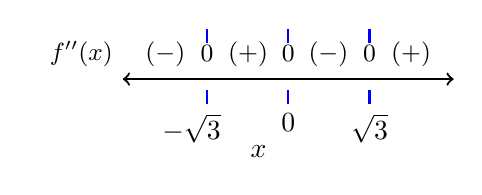
\begin{tikzpicture}[scale=1]
              \begin{axis}[
              axis y line=left,
            xlabel={$x$},
            ylabel={},
            xlabel style={anchor=west},
	  y axis line style={draw=none},
	  	  x axis line style={draw opacity=0},
            %grid = major,
            every major tick/.append style={ thick, blue, major tick length=5pt},
            xtick       = {-1.72, 0, 1.72},
            xticklabels = {$-\sqrt{3}\;\;\;\;$ ,$0$,  $\sqrt{3}$},
            ytick       = \empty,
            yticklabels={},
                                      y  axis line style=-,
                          % y axis/.append style={y axis line style=-}
            samples     = 320,
            restrict y to domain=-40:40,
            xmin = -5.5, xmax = 3.5,
            ymin = -.5, ymax = 1,
            height=1in, width=2.75in
          ]
	\draw[thick,<->] (-3.5,0) -- (3.5,0);
	 \node[anchor=west] at (-5.25,.5) {\small $f^{\prime\prime}(x)$};
	  \node at (-1.72,.5) {\small $0$};
	  	   \node at (0,.5) {\small $0$};
	   \node at (1.72,.5) {\small $0$};
		\node at (-2.6,.5) {\small $(-)$};
		\node at (-.85,.5) {\small $(+)$};
		\node at (.85,.5) {\small $(-)$};
		\node at (2.6,.5) {\small $(+)$};
          %
        \end{axis}
    \end{tikzpicture}
\end{center}
\item At $x=-1$, $f^{\prime\prime}(-1)>0$ so by Second Derivative Test, we have a local minimum.
\item At $x=1$, $f^{\prime\prime}(1)<0$ so by Second Derivative Test, we have a local maximum.

}
}
    
}

%%%%%%%%%
\newpage%
%%%%%%%%%

\paragraph*{Note:} The following problem is based on a problem appearing on an exam during the Fall 2023 semester.\\\\
{\bf\color{blue}Exam Practice 1.}\ltrm{\color{RedOrange}A1} What would the $x$-coordinates of inflection points on the graph of $f$ be if....  \\
Justify your answers using relevant definitions or properties from the first page of this activity.

\mpageT{.5}{.5}{
\enumA{\item the curve pictured to the right is the graph of $f$?}
\sol{
Given the graph of $f$, we're looking for where concavity changes sign and graph changes from bending up to bending down or vice-versa.  \\\\
This appears to happen around $x=3$ and $x=6$.
}
}{
\begin{flushright}
    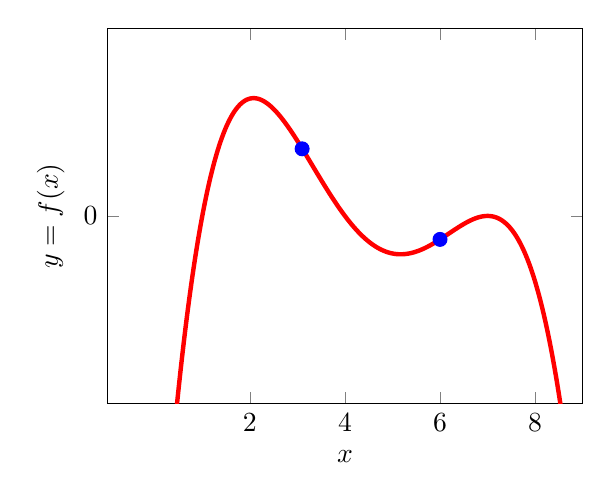
\begin{tikzpicture}[scale=1]
          \begin{axis}[
            xlabel={$x$},
		ylabel={$y=f(x)$},
            %grid = major,
            xtick       = {2,4,6,8},
            xticklabels = {$2$,$4$,$6$,$8$},
            ytick       = {0},
            yticklabels = {$0$},
            samples     = 320,
            domain      = -1:9,
            restrict y to domain=-40:40,
            xmin = -1, xmax = 9,
            ymin = -4, ymax = 4,
            height=2.5in, width=3in
          ]
          % old version of the curve
          %
          %\addplot[domain=-1:9, purple, ultra thick, mark=none] {-1/10*(x-1)*(x-4)^2*(x-7)};
          %
          %new version of the curve in pieces
          %
%          \addplot[domain=-1:3, ultra thick, red] {-(x-2)^2};
%          \addplot[domain=3:4, ultra thick, red] {(x-4)^2-2};
%          \addplot[domain=4:5, ultra thick, red] {2*(x-4)^2-2};
%          \addplot[domain=5:9, ultra thick, red] {-2*(x-6)^2+2};
          %
          %even newer
            \addplot[domain=-1:9, purple, ultra thick, red, mark=none] {-1/20*(x-1)*(x-4)*(x-7)^2};
            \filldraw[blue] (3.1,1.43) circle (2.5pt);
              \filldraw[blue] (6,-.5) circle (2.5pt);
        \end{axis}
    \end{tikzpicture}
\end{flushright}
}
\vfill

\mpageT{.5}{.5}{
\enumA{\setItemnumber{2} \item the curve pictured to the right is the graph of $f'$?}
\sol{
Given the graph of $f^{\prime}$ we know the (unseen) graph of $f$ will be concave up when $f^{\prime}$ is increasing.We  know the (unseen) graph of $f$ will be concave down when $f^{\prime}$ is decreasing. Thus an inflection point will occur when $f^{\prime}$ changes from increasing to decreasing or vice/versa.\\\\
This appears to happen at $x=2$, $x=5$ and $x=7$.
}
}{
\begin{flushright}
    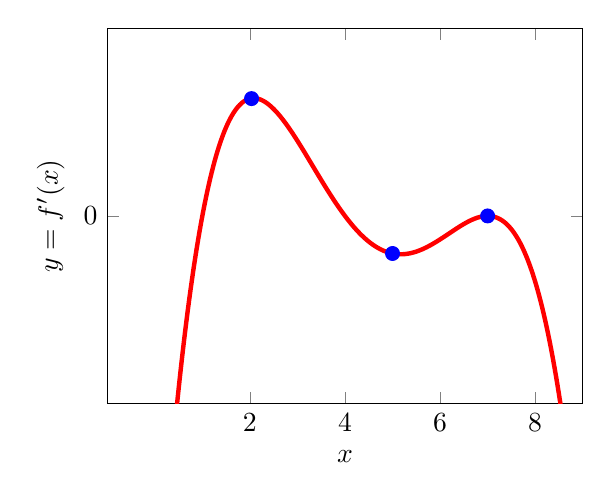
\begin{tikzpicture}[scale=1]
          \begin{axis}[
            xlabel={$x$},
		ylabel={$y=f^{\prime}(x)$},
            %grid = major,
            xtick       = {2,4,6,8},
            xticklabels = {$2$,$4$,$6$,$8$},
            ytick       = {0},
            yticklabels = {$0$},
            samples     = 320,
            domain      = -1:9,
            restrict y to domain=-40:40,
            xmin = -1, xmax = 9,
            ymin = -4, ymax = 4,
            height=2.5in, width=3in
          ]
          % old version of the curve
          %
          %\addplot[domain=-1:9, purple, ultra thick, mark=none] {-1/10*(x-1)*(x-4)^2*(x-7)};
          %
          %new version of the curve in pieces
          %
%          \addplot[domain=-1:3, ultra thick, red] {-(x-2)^2};
%          \addplot[domain=3:4, ultra thick, red] {(x-4)^2-2};
%          \addplot[domain=4:5, ultra thick, red] {2*(x-4)^2-2};
%          \addplot[domain=5:9, ultra thick, red] {-2*(x-6)^2+2};
          %
            %even newer
		\addplot[domain=-1:9, purple, ultra thick, red, mark=none] {-1/20*(x-1)*(x-4)*(x-7)^2};
		\filldraw[blue] (2.035,2.5) circle (2.5pt);
		\filldraw[blue] (5,-.8) circle (2.5pt);
		\filldraw[blue] (7,0) circle (2.5pt);
        \end{axis}
    \end{tikzpicture}
\end{flushright}
}
\vfill

 \mpageT{.5}{.5}{
\enumA{\setItemnumber{3} \item the curve pictured to the right is the graph of $f''$?}
\sol{
Given the graph of $f^{\prime\prime}$ we know the (unseen) graph of $f$ will be concave up when $f^{\prime\prime}>0$ and will be concave down when $f^{\prime\prime}<0$. Inflection points occur when the sign of $f^{\prime\prime}$  changes from positive to negative or vice versa.  \\\\
This appears to occur    at $x=1$ and $x=4$ only.\\\\
Note that $x=7$ is {\em not} an inflection point because the graph does not change from negative to positive there.
}
}{
\begin{flushright}
    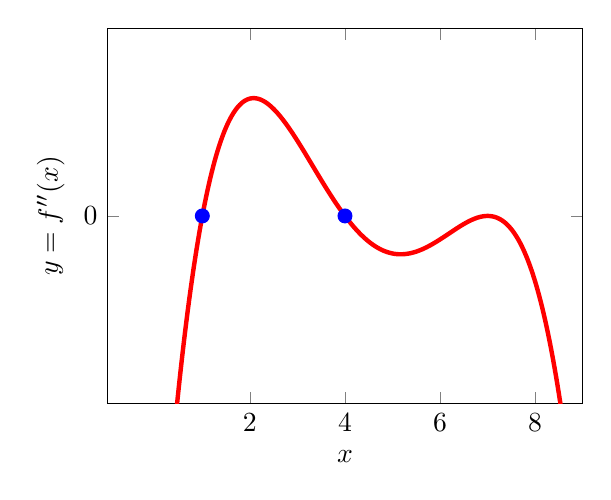
\begin{tikzpicture}[scale=1]
          \begin{axis}[
            xlabel={$x$},
		ylabel={$y=f^{\prime\prime}(x)$},
            %grid = major,
            xtick       = {2,4,6,8},
            xticklabels = {$2$,$4$,$6$,$8$},
            ytick       = {0},
            yticklabels = {$0$},
            samples     = 320,
            domain      = -1:9,
            restrict y to domain=-40:40,
            xmin = -1, xmax = 9,
            ymin = -4, ymax = 4,
            height=2.5in, width=3in
          ]
          % old version of the curve
          %
          %\addplot[domain=-1:9, purple, ultra thick, mark=none] {-1/10*(x-1)*(x-4)^2*(x-7)};
          %
          %new version of the curve in pieces
          %
%          \addplot[domain=-1:3, ultra thick, red] {-(x-2)^2};
%          \addplot[domain=3:4, ultra thick, red] {(x-4)^2-2};
%          \addplot[domain=4:5, ultra thick, red] {2*(x-4)^2-2};
%          \addplot[domain=5:9, ultra thick, red] {-2*(x-6)^2+2};
          %
            %even newer
            \addplot[domain=-1:9, purple, ultra thick, red, mark=none] {-1/20*(x-1)*(x-4)*(x-7)^2};
            		\filldraw[blue] (1,0) circle (2.5pt);
		\filldraw[blue] (4,0) circle (2.5pt);
        \end{axis}
    \end{tikzpicture}
\end{flushright}
}
\vfill



%%%%%%%%%
\newpage%
%%%%%%%%%

{\bf\color{blue} Extra Practice 1.} Let $g(x)=x^{2/3}(x+2)$. You may take as given that $g'(x)=\dfrac{5x+4}{3\sqrt[3]{x}}$ and $g''(x)=\dfrac{2(5x-2)}{9x^{4/3}}$.
\enumA{
\item\ltrm{\color{RedOrange}A1} Find the intervals where the graph of $g$ is concave up and concave down.
\sol{ We will build a sign line starting with \\
\blue{
\mpageT{.5}{.5}[\vline\hs{.05}]{\vs{-.2}
\al{
g^{\prime\prime}(x)&=0\\
\frac{2(5x-2)}{9x^{4/3}}&=0
\intertext{We focus on the numerator}
2(5x-2)&=0\\
5x-2&=0\\
5x&=2\\
x=\frac{2}{5}
}
We also notice that when $x=0$, $9\cdot (0)^{4/3}=0$ and thus  $\ds g^{\prime\prime}(0)=\dfrac{2(5\cdot 0-2)}{0}$ does not exist at $x=0$. Thus $x=0$ is also a candidate for an inflection point.    We begin our sign line: 
\begin{center}
\begin{tikzpicture}[scale=1]
              \begin{axis}[
              axis y line=left,
            xlabel={$x$},
            ylabel={},
            xlabel style={anchor=west},
	  y axis line style={draw=none},
	  	  x axis line style={draw opacity=0},
            %grid = major,
            every major tick/.append style={ thick, blue, major tick length=5pt},
            xtick       = { 0, .4},
            xticklabels = { $0$,  $\frac{2}{5}$},
            ytick       = \empty,
            yticklabels={},
                                      y  axis line style=-,
                          % y axis/.append style={y axis line style=-}
            samples     = 320,
            restrict y to domain=-40:40,
            xmin = -.65, xmax = .8,
            ymin = -.5, ymax = 1,
            height=1in, width=2.75in
          ]
	\draw[thick,<->] (-.4,0) -- (.8,0);
	 \node[anchor=west] at (-.65,.5) {\small $g^{\prime\prime}(x)$};
	  	   \node at (0,.5) {\small $0$};
	   \node at (.4,.5) {\small $0$};
%		\node at (-2.6,.5) {\small $(-)$};
%		\node at (-.85,.5) {\small $(+)$};
%		\node at (.85,.5) {\small $(-)$};
%		\node at (2.6,.5) {\small $(+)$};
          %
        \end{axis}
    \end{tikzpicture}
\end{center}
}{
We test values from each interval created by the sign line.
\itemI{
\item Choose a point in $x<0$, say $x=-1$.$$ g^{\prime\prime}(-1)=\frac{2(5(-1)-2)}{9(-1)^{4/3}}=\frac{2\cdot(-7)}{9\cdot \sqrt[3]{(-1)^4}}=\frac{-14}{9\sqrt[3]{1}}<0$$
\item Choose a point in $0<x<2/5$, say $x=1/5$.$$ g^{\prime\prime}(1/5)=\frac{2(5(1/5)-2)}{9(1/5)^{4/3}}=\frac{2\cdot(-1)}{9(1/5)^{4/3}}=\frac{(-)}{(+)}<0$$
\item Choose a point in $x>2/5$, say $x=-1$.$$ g^{\prime\prime}(1)=\frac{2(5(1)-2)}{9(1)^{4/3}}=\frac{6}{9}>0$$
}
We update our sign line: 
\begin{center}
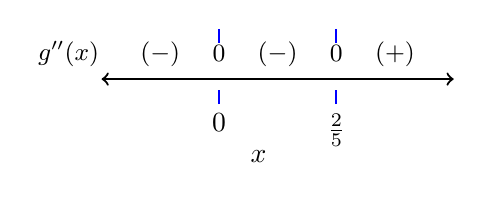
\begin{tikzpicture}[scale=1]
              \begin{axis}[
              axis y line=left,
            xlabel={$x$},
            ylabel={},
            xlabel style={anchor=west},
	  y axis line style={draw=none},
	  	  x axis line style={draw opacity=0},
            %grid = major,
            every major tick/.append style={ thick, blue, major tick length=5pt},
            xtick       = {  0, .4},
            xticklabels = { $0$, $\frac{2}{5}$},
            ytick       = \empty,
            yticklabels={},
                                      y  axis line style=-,
                          % y axis/.append style={y axis line style=-}
            samples     = 320,
            restrict y to domain=-40:40,
            xmin = -.65, xmax = .8,
            ymin = -.5, ymax = 1,
            height=1in, width=2.75in
          ]
	\draw[thick,<->] (-.4,0) -- (.8,0);
	 \node[anchor=west] at (-.65,.5) {\small $g^{\prime\prime}(x)$};
	  	   \node at (0,.5) {\small $0$};
	   \node at (.4,.5) {\small $0$};
		\node at (-.2,.5) {\small $(-)$};
		\node at (.2,.5) {\small $(-)$};
		\node at (.6,.5) {\small $(+)$};
          %
        \end{axis}
    \end{tikzpicture}
\end{center}
}
}~\\\\
Based on our updated sign line:
\itemI{
\item Concave up intervals are $(1,\infty)$
\item Concave down intervals are $(-\infty,0),\, (0,2/5)$
}
}


\item\ltrm{\color{RedOrange}A1} Specify the $x$-coordinates of any inflection points on the graph of $g$.
\sol{
Based on sign line from previous problem we see that $g^{\prime\prime}$ changes sign only at $\ds x=\frac{2}{5}$. This is our only inflection point.
}



\item\ltrm{\color{RedOrange}A2} What does the Second Derivative Test tell us about the behavior of $g$ at its critical numbers?
\sol{
We first find our critical numbers.
\al{
g^{\prime}(x)&=0\\
\frac{5x+4}{3\sqrt[3]{x}}&=0
\intertext{We first focus on the numerator.}
5x+4&=0\\
5x&=-4\\
x&=-\frac{4}{5}
\intertext{We next focus on the denominator to see if is equal to $0$ as this would mean  $g^{\prime}=DNE$. }
3\sqrt[3]{x}&=0\\
x^{1/3}&=0\\
x&=0
}
We have two critical numbers: $\ds x= -\frac{4}{5},\, 0$.
\itemI{
\item Based on our sign line in part a), $g^{\prime\prime}(-4/5)<0$. The Second Derivative Test tells us that this means we have a local maximum.
\item Since $g^{\prime}(0) = DNE$, we cannot use the Second Derivative Test.  But we {\em can} use the First Derivative test. Our initial sign line is:
\begin{center}
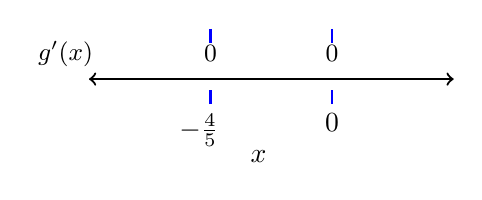
\begin{tikzpicture}[scale=1]
              \begin{axis}[
              axis y line=left,
            xlabel={$x$},
            ylabel={},
            xlabel style={anchor=west},
	  y axis line style={draw=none},
	  	  x axis line style={draw opacity=0},
            %grid = major,
            every major tick/.append style={ thick, blue, major tick length=5pt},
            xtick       = {  -.8, 0},
            xticklabels = { $-\frac{4}{5}\;\;\;$,$0$ },
            ytick       = \empty,
            yticklabels={},
                                      y  axis line style=-,
                          % y axis/.append style={y axis line style=-}
            samples     = 320,
            restrict y to domain=-40:40,
            xmin = -2, xmax = .8,
            ymin = -.5, ymax = 1,
            height=1in, width=2.75in
          ]
	\draw[thick,<->] (-1.6,0) -- (.8,0);
	 \node[anchor=west] at (-2,.5) {\small $g^{\prime}(x)$};
	  	   \node at (0,.5) {\small $0$};
	   \node at (-.8,.5) {\small $0$};
%		\node at (-.2,.5) {\small $(-)$};
%		\node at (.2,.5) {\small $(-)$};
%		\node at (.6,.5) {\small $(+)$};
          %
        \end{axis}
    \end{tikzpicture}
\end{center}

Since we already know we have a local maximum at $\ds x=-\frac{4}{5}$, we're going to focus on the critical number $x=0$.  
\itemI{
\item Choose a value in $-4/5<x<0$, say $\ds x=-\frac{2}{5}$
\al{
g^{\prime}(-2/5)&=\frac{5(-2/5)+4}{3\cdot (-\frac{2}{5})^{1/3}}\\
&=\frac{-2+4}{3\cdot (-\frac{2}{5})^{1/3}}
\intertext{The cube root of a negative number is negative. Thus in the denominator $ \left(-\frac{2}{5}\right)^{1/3}<0$ }
&=\frac{(+)}{(-)}\\
g^{\prime}(-2/5)&<0
}
\item Choose a value in $x>0$, say $x=1$.
\al{
g^{\prime}(1)&=\frac{5\cdot 1+4}{3\cdot (1)^{1/3}}\\
&=\frac{9}{3}\\
g^{\prime}(1)&>0
} 
We update our sign line:
\begin{center}
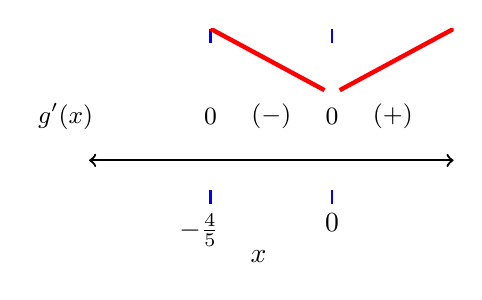
\begin{tikzpicture}[scale=1]
              \begin{axis}[
              axis y line=left,
            xlabel={$x$},
            ylabel={},
            xlabel style={anchor=west},
	  y axis line style={draw=none},
	  	  x axis line style={draw opacity=0},
            %grid = major,
            every major tick/.append style={ thick, blue, major tick length=5pt},
            xtick       = {  -.8, 0},
            xticklabels = { $-\frac{4}{5}\;\;\;$,$0$ },
            ytick       = \empty,
            yticklabels={},
                                      y  axis line style=-,
                          % y axis/.append style={y axis line style=-}
            samples     = 320,
            restrict y to domain=-40:40,
            xmin = -2, xmax = .8,
            ymin = -.5, ymax = 1.5,
            height=1.5in, width=2.75in
          ]
	\draw[thick,<->] (-1.6,0) -- (.8,0);
	 \node[anchor=west] at (-2,.5) {\small $g^{\prime}(x)$};
	  	   \node at (0,.5) {\small $0$};
	   \node at (-.8,.5) {\small $0$};
		\node at (-.4,.5) {\small $(-)$};
		\node at (.4,.5) {\small $(+)$};
		\draw[ultra thick, red] (-.8,1.5) -- (-.05,.8);
		\draw[ultra thick, red] (.05,.8) -- (.8,1.5);
          %
        \end{axis}
    \end{tikzpicture}
\end{center}
}
Thus $g(x)$ decreases approaching $x=0$ from the left and increases as we move to the right off $x=0$. This means we have a local minimum.
}
}
}


\end{document}
